\documentclass[hyperref, a4paper]{article}

\usepackage{geometry}
\usepackage{float}
\usepackage{titling}
\usepackage{titlesec}
% No longer needed, since we will use enumitem package
% \usepackage{paralist}
\usepackage{enumitem}
\usepackage{footnote}
\usepackage{enumerate}
\usepackage{amsmath, amssymb, amsthm}
\usepackage{mathtools}
\usepackage{bbm}
\usepackage{cite}
\usepackage{graphicx}
\usepackage{subcaption}
\usepackage{physics}
\usepackage{tensor}
\usepackage{siunitx}
\usepackage{booktabs}
\usepackage[version=4]{mhchem}
\usepackage{tikz}
\usepackage{xcolor}
\usepackage{listings}
\usepackage{autobreak}
\usepackage[ruled, vlined, linesnumbered]{algorithm2e}
\usepackage{xr-hyper}
\usepackage[colorlinks,unicode]{hyperref} % , linkcolor=black, anchorcolor=black, citecolor=black, urlcolor=black, filecolor=black
\usepackage{prettyref}

% Page style
\geometry{left=3.18cm,right=3.18cm,top=2.54cm,bottom=2.54cm}
\titlespacing{\paragraph}{0pt}{1pt}{10pt}[20pt]
\setlength{\droptitle}{-5em}
\preauthor{\vspace{-10pt}\begin{center}}
\postauthor{\par\end{center}}

% More compact lists 
\setlist[itemize]{itemindent=17pt, leftmargin=1pt}

% Math operators
\DeclareMathOperator{\timeorder}{\mathcal{T}}
\DeclareMathOperator{\diag}{diag}
\DeclareMathOperator{\legpoly}{P}
\DeclareMathOperator{\primevalue}{P}
\DeclareMathOperator{\sgn}{sgn}
\newcommand*{\ii}{\mathrm{i}}
\newcommand*{\ee}{\mathrm{e}}
\newcommand*{\const}{\mathrm{const}}
\newcommand*{\suchthat}{\quad \text{s.t.} \quad}
\newcommand*{\argmin}{\arg\min}
\newcommand*{\argmax}{\arg\max}
\newcommand*{\normalorder}[1]{: #1 :}
\newcommand*{\pair}[1]{\langle #1 \rangle}
\newcommand*{\fd}[1]{\mathcal{D} #1}
\DeclareMathOperator{\bigO}{\mathcal{O}}
\DeclareMathOperator{\object}{Ob}
\DeclareMathOperator{\morphism}{Hom}

% TikZ setting
\usetikzlibrary{arrows,shapes,positioning}
\usetikzlibrary{arrows.meta}
\usetikzlibrary{decorations.markings}
\tikzstyle arrowstyle=[scale=1]
\tikzstyle directed=[postaction={decorate,decoration={markings,
    mark=at position .5 with {\arrow[arrowstyle]{stealth}}}}]
\tikzstyle ray=[directed, thick]
\tikzstyle dot=[anchor=base,fill,circle,inner sep=1pt]

% Algorithm setting
% Julia-style code
\SetKwIF{If}{ElseIf}{Else}{if}{}{elseif}{else}{end}
\SetKwFor{For}{for}{}{end}
\SetKwFor{While}{while}{}{end}
\SetKwProg{Function}{function}{}{end}
\SetArgSty{textnormal}

\newcommand*{\concept}[1]{{\textbf{#1}}}

\newrefformat{fig}{Figure~\ref{#1}}

% Embedded codes
\lstset{basicstyle=\ttfamily,
  showstringspaces=false,
  commentstyle=\color{gray},
  keywordstyle=\color{blue}
}

\title{Quantum Optics, Homework 2}
\author{Jinyuan Wu}

\begin{document}

\maketitle

\begin{figure}
    \centering
    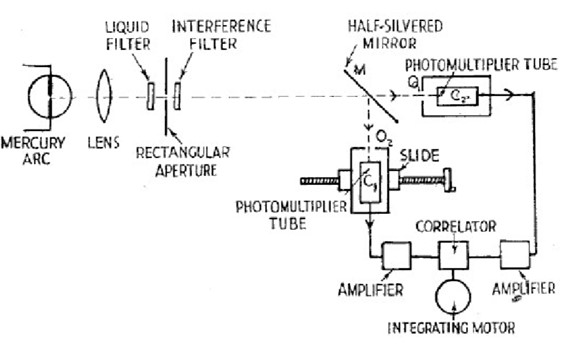
\includegraphics[width=0.65\textwidth]{hbt-lab.png}
    \caption{HBT effect in laboratory}
    \label{fig:hbt-lab}
\end{figure}

\begin{figure}
    \centering
    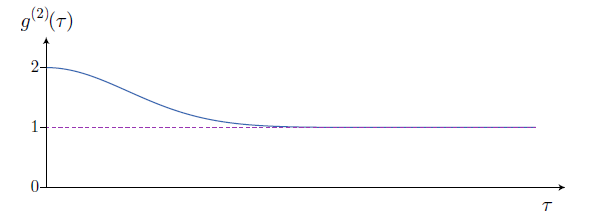
\includegraphics[width=0.6\textwidth]{thermal-state-g2.PNG}
    \caption{Second order coherence with a thermal light source in Gaussian distribution (figure taken from \cite{optical-note-steck}, Section~2.6.1).
    The maximum of $g^{(2)}$ is 2, which is a result of the optical field obeying a Gaussian distribution, where the Wick theorem holds so $\expval{E^*_1 E^*_2 E_3 E_4} = \expval{E^*_1 E_3} \expval{E^*_2 E_4} + \expval{E^*_1 E_4} \expval{E^*_2 E_3}$, and hence $\expval*{I^2} = 2 \expval{I}^2$.}
    \label{fig:thermal-hbt}
\end{figure}

\paragraph{Details in the HBT experiment} \prettyref{fig:hbt-lab} shows an experimental validation of the HBT effect. 
(a) Describe the expected phenomenon the experiment. Compare the expected phenomenon with the original HBT effect in astronomical observation.
(b) Explain the phenomenon within classical electrodynamics.
(c) Point out why the classical explanation is not enough. Construct a simplified version of the experiment and explain it with quantum optics.

\paragraph{Solution} \begin{itemize}
    \item[(a)] The integrating motor gives the averaged intensity correlation function, i.e.
    \begin{equation}
        \expval*{I_1 I_2} \coloneqq \lim_{T \to \infty} \frac{1}{T} \int_0^T \dd{t} I_1(t) I_2(t). 
    \end{equation} 
    The expected results include that
    \begin{equation}
        \expval*{I_1 I_2} - \expval{I_1} \expval{I_2} \neq 0, \quad g^{(2)} > 1,
    \end{equation} 
    and that the intensity fluctuation correlation function 
    \begin{equation}
        \expval{\Delta I_1 \Delta I_2} = \expval*{I_1 I_2} - \expval{I_1} \expval{I_2}
    \end{equation}
    reaches its peak when the optical path difference of the two beams is zero, and then drops away as the separation between the two beams increases. 
    If the light source is laser, the relation between $g^{(2)}$ and the optical path difference is in the form of $1 + A \cos(k \Delta r)$, while if the light source is thermal - as is the case of a mercury arc - the relation between $g^{(2)}$ and the optical path separation is something like \prettyref{fig:thermal-hbt}.
    \item[(b)] Suppose the electric field before the beam splitter is $E(t) \cos(\omega t)$, where the characteristic frequency of $E(t)$ is much smaller than $\omega$.
    The beam splitter introduces a phase difference of $\pi$ between the reflected beam and the transmitted beam, and the fact that $MO_1$ may be different with $MO_2$ introduces another phase difference.
    The electric fields at detecter 1 and detecter 2 are therefore 
    \begin{equation}
        E_1 = E(t - \tau_1) \cos(\omega (t - \tau_1)), \quad E_2 = E(t - \tau_2) \cos(\omega (t - \tau_2)),
    \end{equation}
    respectively.
    The intensities of $E_1$ and $E_2$ are 
    \begin{equation}
        I_1(t) = \overline{E(t - \tau_1)^2 \cos^2 \omega(t - \tau_1)} = \frac{1}{2} E(t - \tau_1)^2, \quad I_2(t) = \frac{1}{2} E(t - \tau_2)^2.
    \end{equation}
    The correlation function is therefore 
    \begin{equation}
        \expval{I_1 I_2} = \expval*{ I_1(t) I_2(t) } = \frac{1}{4} \expval*{E(t - \tau_1)^2 E(t - \tau_2)^2}.
    \end{equation}
    
    With a thermal light source, when $\abs*{\tau_1 - \tau_2}$ is large, $E(t - \tau_1)$ and $E(t - \tau_2)$ is not correlated, and we have 
    \[
        g^{(2)} = \frac{\expval{I_1 I_2}}{\expval{I_1} \expval{I_2}} \approx \frac{\expval{I_1} \expval{I_2}}{\expval{I_1} \expval{I_2}} = 1.
    \]
    When $\tau_1 = \tau_2$, however, we have 
    \[
        \expval{(I_1(t) - \expval*{I_1}) (I_2(t) - \expval*{I_2})} > 0,
    \]
    and subsequently
    \[
        \expval*{I_1 I_2} - \expval*{I_1} \expval*{I_2} > 0, 
    \]
    so $g^{(2)} > 1$.
    So we have something like \prettyref{fig:thermal-hbt}.
    \item[(c)] When the classical picture of the optical field fails, the classical explanation fails as well.
    For example, when the light source creates a sequence of single-photon pulses, what will be observed is \emph{photon antibunching} where $g^{(2)} = 0$ instead of bunching, because one photon cannot appear at two sites.
\end{itemize}

\begin{figure}
    \centering
    

\tikzset{every picture/.style={line width=0.75pt}} %set default line width to 0.75pt        

\begin{tikzpicture}[x=0.75pt,y=0.75pt,yscale=-1,xscale=1]
%uncomment if require: \path (0,335); %set diagram left start at 0, and has height of 335

%Shape: Circle [id:dp520440537429514] 
\draw  [draw opacity=0][fill={rgb, 255:red, 255; green, 255; blue, 0 }  ,fill opacity=1 ] (276.44,17.09) .. controls (276.44,12.63) and (280.06,9.01) .. (284.53,9.01) .. controls (288.99,9.01) and (292.61,12.63) .. (292.61,17.09) .. controls (292.61,21.56) and (288.99,25.17) .. (284.53,25.17) .. controls (280.06,25.17) and (276.44,21.56) .. (276.44,17.09) -- cycle ;
%Straight Lines [id:da6010958544087177] 
\draw [color={rgb, 255:red, 208; green, 2; blue, 27 }  ,draw opacity=1 ]   (277.39,16.09) -- (318,198.33) ;
\draw [shift={(297.7,107.21)}, rotate = 257.44] [fill={rgb, 255:red, 208; green, 2; blue, 27 }  ,fill opacity=1 ][line width=0.08]  [draw opacity=0] (12,-3) -- (0,0) -- (12,3) -- cycle    ;
%Straight Lines [id:da5792212007108453] 
\draw [color={rgb, 255:red, 74; green, 144; blue, 226 }  ,draw opacity=1 ]   (292.61,16.09) -- (318,198.33) ;
\draw [shift={(305.3,107.21)}, rotate = 262.07] [fill={rgb, 255:red, 74; green, 144; blue, 226 }  ,fill opacity=1 ][line width=0.08]  [draw opacity=0] (12,-3) -- (0,0) -- (12,3) -- cycle    ;
%Straight Lines [id:da7563818948167416] 
\draw [color={rgb, 255:red, 208; green, 2; blue, 27 }  ,draw opacity=1 ]   (277.39,16.09) -- (266,197.33) ;
\draw [shift={(271.7,106.71)}, rotate = 273.6] [fill={rgb, 255:red, 208; green, 2; blue, 27 }  ,fill opacity=1 ][line width=0.08]  [draw opacity=0] (12,-3) -- (0,0) -- (12,3) -- cycle    ;
%Straight Lines [id:da6535572732710992] 
\draw [color={rgb, 255:red, 74; green, 144; blue, 226 }  ,draw opacity=1 ]   (292.61,17.09) -- (266,198.33) ;
\draw [shift={(279.3,107.71)}, rotate = 278.35] [fill={rgb, 255:red, 74; green, 144; blue, 226 }  ,fill opacity=1 ][line width=0.08]  [draw opacity=0] (12,-3) -- (0,0) -- (12,3) -- cycle    ;
%Shape: Rectangle [id:dp9534783904946957] 
\draw   (257.33,198.11) -- (274.67,198.11) -- (274.67,208.44) -- (257.33,208.44) -- cycle ;
%Straight Lines [id:da19171375211786357] 
\draw    (243.33,208.58) -- (334.33,208.58) ;
%Shape: Rectangle [id:dp4919024765051321] 
\draw   (307.33,198.11) -- (324.67,198.11) -- (324.67,208.44) -- (307.33,208.44) -- cycle ;
%Curve Lines [id:da3025737714669319] 
\draw    (266,208.28) .. controls (220,236.67) and (231,251.67) .. (263,262.67) ;
%Shape: Rectangle [id:dp550560509737535] 
\draw   (263,247.67) -- (314,247.67) -- (314,276) -- (263,276) -- cycle ;

%Curve Lines [id:da6860861023811542] 
\draw    (317.17,209.28) .. controls (363.17,237.67) and (346,252.67) .. (314,263.67) ;

% Text Node
\draw (268.75,210.4) node [anchor=north] [inner sep=0.75pt]    {$I_{1}$};
% Text Node
\draw (310.25,210.4) node [anchor=north west][inner sep=0.75pt]    {$I_{2}$};
% Text Node
\draw (288.5,261.83) node    {$\langle I_{1} I_{2} \rangle $};


\end{tikzpicture}

    \caption{HBT in astronomical observation}
    \label{fig:hbt-astronomy}
\end{figure}

\paragraph{}

\paragraph{Conditional generation of single photon pulses} Many research and applications in quantum optics needs single photon pulses, that is, a wave packet of light that contains exactly one single photon. Such a single photon pulse can be generated in two ways: The deterministic approach via single atom emission, and the so-called heralded approach. This problem discusses a simplified version of the later.
Consider a bi-photon generation process described by the Hamiltonian  
\begin{equation}
    H=\beta a_{k}^\dagger b_{k^{\prime}}^\dagger+ \text{h.c.}.
\end{equation}
Here $a_{k}^\dagger, b_{k^{\prime}}^\dagger$ are creation operators of photons into the $k, k'$ propagation modes respectively. Such process can be realized for example in a frequency down conversion experiment, where a single photon is ``split'' into two in a nonlinear optical crystal, or a 4-wave mixing experiment where two incoming photons are converted into two output photons in an atomic gas.
(a) Consider initially light is in vacuum state $|\psi(0)\rangle=|V\rangle$. Consider that the bi-photon generation process is switched on for time $\tau$ and then off, with $\xi=\beta \tau \ll 1$. Integrate the Schrodinger equation to obtain $|\psi(\tau)\rangle$, that is, the photon state after the interaction. (b) Consider a photon detector positioned $L$ meters away from the bi-photon generation device along the $k'$ propagation pathway. The time interval that the detector can detect a $b_{k'}$ photon is $[L / c, L / c+\tau]$ (we ignore any change of light speed within the experiment). For an ideal photon detector, what is the probability of detecting 1 photon, and detecting 2 photons during this time interval? If one photon is detected along $k'$, what is the photon state in the $k$ path? The strategy is the so called heralded single photon generation: a nearly perfect single photon pulse in the $k$ mode is heralded by the detection of a single photon in the $k'$-mode.

\paragraph{Solution} \begin{itemize}
    \item[(a)] In the interaction picture, the time evolution of the state is given by
    \[
        \ii \dv{t} \ket*{\psi(t)} = H \ket*{\psi(t)} = h(t) \left( \beta a^\dagger_{k} b_{k'}^\dagger + \text{h.c.} \right) \ket*{\psi(t)},
    \] 
    where $h(t)$ is one when $t \in [0, \tau]$ and zero otherwise.
    Formally we have 
    \[
        \ket*{\psi(t)} = \timeorder \exp(- \ii \int_0^t \dd{t'} h(t') (\beta a^\dagger_k b^\dagger_{k'} + \text{h.c.})) \ket*{\psi(0)}.
    \]
    Since $\xi \ll 1$, the operators approximately do not have time evolution, and thus we have 
    \begin{equation}
        \begin{aligned}
            \ket*{\psi(\tau)} &= \exp(- \ii \tau (\beta a^\dagger_k b^\dagger_{k'} + \text{h.c.})) \ket*{\psi(0)} \\
            &= \ee^{- \ii \xi (a^\dagger_k b^\dagger_{k'} + a_k b_{k'})} \ket*{0} .
        \end{aligned}
        \label{eq:final-state-tau}
    \end{equation}
    \item[(b)] Since the time interval is very short, we can view the measurement as simply measuring the state \eqref{eq:final-state-tau} as the pulse comes across the detector.
    Expanding \eqref{eq:final-state-tau} we have 
    \[
        \begin{aligned}
            \ket*{\psi(\tau)} &= \ket*{0} - \ii \xi (a^\dagger_{k} b^\dagger_{k'} + \text{h.c.}) \ket*{0} + \frac{1}{2} (- \ii \xi)^2 (a^\dagger_{k} b^\dagger_{k'} + \text{h.c.})^2 \ket*{0} + \cdots \\
            &= \left( 1 - \frac{\xi^2}{2} + \cdots \right) \ket*{0} - (\ii \xi + \cdots) \ket*{n_k = 1, n_{k'} = 1} - \left( \frac{1}{2} \xi^2 + \cdots \right) \ket*{n_k = 2, n_{k'} = 2} + \cdots.  
        \end{aligned}
    \] 
    Taking only the leading order terms, we have 
    \begin{equation}
        P(n_k = 1) = \xi^2, \quad P(n_k = 2) = \frac{\xi^4}{4}.
    \end{equation}

    It can be seen that in $\ket*{\psi(\tau)}$ we always have $n_k = n_{k'}$, and therefore if one photon is detected along $k'$, the photon state in the $k$ path is $\ket*{n_k = 1}$.
    Therefore if we placed a baffle in path $k$, which is removed when $n_{k'}$ is detected to be $1$, whenever a pulse is generated, it is a single-photon one.
\end{itemize}

\begin{figure}
    \centering
    

\tikzset{every picture/.style={line width=0.75pt}} %set default line width to 0.75pt        

\begin{tikzpicture}[x=0.75pt,y=0.75pt,yscale=-1,xscale=1]
%uncomment if require: \path (0,300); %set diagram left start at 0, and has height of 300

%Shape: Rectangle [id:dp9291562475809372] 
\draw  [draw opacity=0][fill={rgb, 255:red, 0; green, 0; blue, 0 }  ,fill opacity=0.36 ] (144,109) -- (165.71,109) -- (165.71,177.67) -- (144,177.67) -- cycle ;
%Straight Lines [id:da8833130318893516] 
\draw    (69.71,142.67) -- (144.71,142.67) ;
\draw [shift={(107.21,142.67)}, rotate = 180] [fill={rgb, 255:red, 0; green, 0; blue, 0 }  ][line width=0.08]  [draw opacity=0] (12,-3) -- (0,0) -- (12,3) -- cycle    ;
%Straight Lines [id:da6688023135314647] 
\draw    (164.85,143.34) -- (239.71,106.67) ;
\draw [shift={(202.28,125.01)}, rotate = 513.9] [fill={rgb, 255:red, 0; green, 0; blue, 0 }  ][line width=0.08]  [draw opacity=0] (12,-3) -- (0,0) -- (12,3) -- cycle    ;
%Straight Lines [id:da8843982354889979] 
\draw    (164.85,143.34) -- (278,186.29) ;
\draw [shift={(221.43,164.81)}, rotate = 200.79] [fill={rgb, 255:red, 0; green, 0; blue, 0 }  ][line width=0.08]  [draw opacity=0] (12,-3) -- (0,0) -- (12,3) -- cycle    ;
%Shape: Chord [id:dp20648494743318113] 
\draw   (283.31,171.99) .. controls (291.94,175.15) and (296.75,183.92) .. (294.07,191.77) .. controls (291.36,199.74) and (281.96,203.75) .. (273.08,200.72) -- cycle ;

% Text Node
\draw (241.71,103.27) node [anchor=south west] [inner sep=0.75pt]    {$k$};
% Text Node
\draw (234.71,174.07) node [anchor=north west][inner sep=0.75pt]    {$k'$};
% Text Node
\draw (152.38,103.74) node [anchor=south] [inner sep=0.75pt]   [align=left] {SPDC};


\end{tikzpicture}

    \caption{Light circuit in the heralded approach}
    \label{fig:heralded-circuit}
\end{figure}

\paragraph{}

\paragraph{Details in the NLS process} Analyze the NLS process in detail. 
The circuit is shown in \prettyref{fig:nls}, and the two beam splitters are represented as 
\begin{equation}
    S_1 = \pmqty{\cos \theta & \sin \theta \\
    - \sin \theta & \cos \theta}, \quad S_2 = \pmqty{\cos \sigma & \sin \sigma \\
    - \sin \sigma & \cos \sigma}
\end{equation}
(a) Derive the output quantum state before the measurement.
(b) Find the conditional quantum state with the measurement results shown in \prettyref{fig:nls}.
(c) Find when the NLS process works in terms of $\theta$ and $\sigma$, and the probability of a successful NLS.

\paragraph{Solution} \begin{itemize}
    \item[(a)] The optical circuit is linear its transformation matrix is 
    \begin{equation}
        S = \pmqty{ 1 & 0 & 0 \\ 0 & \cos \sigma & \sin \sigma \\ 0 & - \sin \sigma & \cos \sigma } \pmqty{ \cos \theta & \sin \theta & 0 \\ - \sin \theta & \cos \theta & 0 \\ 0 & 0 & 1  } = \pmqty{ \cos \theta & \sin \theta & 0 \\ - \cos \sigma \sin \theta & \cos \sigma \cos \theta & \sin \sigma \\ \sin \theta \sin \sigma & - \cos \theta \sin \sigma & \cos \sigma },
        \label{eq:s-matrix-nls}
    \end{equation} 
    and we have 
    \begin{equation}
        b^\dagger_j = S_{jk} a^\dagger_k.
        \label{eq:b-a-nls}
    \end{equation}
    The quantum state is 
    \[
        \ket*{\psi} = \big( \alpha + \beta a_1^\dagger + \frac{\gamma}{\sqrt{2}} (a_1^\dagger)^2 \big) a_2^\dagger \ket*{0} .
    \]
    By \eqref{eq:s-matrix-nls} and \eqref{eq:b-a-nls} we have 
    \[
        [a_i]^\dagger = \pmqty{\cos \theta  & -\cos \sigma  \sin \theta  & \sin \theta  \sin \sigma  \\
        \sin \theta  & \cos \theta  \cos \sigma  & -\cos \theta  \sin \sigma  \\
        0 & \sin \sigma  & \cos \sigma  } [b_i^\dagger],
    \]
    and therefore we have 
    \begin{equation}
        \begin{aligned}
            \ket*{\psi} &= \Big( \alpha + \beta ( b_1^\dagger \cos \theta - b_2^\dagger \sin \theta  \cos \sigma + b_3^\dagger \sin \theta  \sin \sigma ) \\
            &\quad \quad + \frac{\gamma}{\sqrt{2}} ( b_1^\dagger \cos \theta - b_2^\dagger \sin \theta  \cos \sigma + b_3^\dagger \sin \theta  \sin \sigma )^2 \Big) \\
            &\quad \times   (b_1^\dagger \sin \theta +b_2^\dagger \cos \theta  \cos \sigma -b_3^\dagger \cos \theta  \sin \sigma ) \ket*{0}.
        \end{aligned}
        \label{eq:nls-psi}
    \end{equation}
    \item[(b)] In \eqref{eq:nls-psi}, the $b_1^\dagger (b_2^\dagger)^0$ terms are
    \[
        \begin{aligned}
            &\quad \alpha b_1^\dagger \sin \theta + \beta b_1^\dagger \cos \theta \times (-b_3^\dagger \cos \theta \sin \sigma) \\
            &+ \beta b_3^\dagger \sin \theta \sin \sigma \times b_1^\dagger \sin \theta \\
            &+ \frac{2 \gamma}{\sqrt{2}} b_1^\dagger \cos \theta \times b_3^\dagger \sin \theta \sin \sigma\times (- b_3^\dagger \cos \theta \sin \sigma) \\
            &+ \frac{\gamma}{\sqrt{2}} (b_3^\dagger)^\dagger \sin^2\theta \sin^2\sigma \times b_1^\dagger \sin \theta,
        \end{aligned}
    \]  
    which also reads 
    \[
        (\alpha \sin\theta + b_3^\dagger \beta \sin\sigma \cos 2 \theta + \frac{1}{\sqrt{2}} (b_3^\dagger)^2 \gamma (\sin^2\theta - 2\cos^2\theta) \sin \theta \sin^2 \sigma) b_1,
    \]
    and therefore the conditional quantum state is 
    \begin{equation}
        \ket*{\psi}_\text{cond-out} = \alpha \sin\theta \ket*{1, 0, 0} + \beta \sin\sigma \cos 2 \theta \ket*{1, 0, 1} + \gamma (\sin^2\theta - 2\cos^2\theta) \sin \theta \sin^2 \sigma \ket*{1, 0, 2}.
        \label{eq:nls-conditional-state}
    \end{equation}
    Note that the state is \emph{not} normalized. Its norm gives the probability to obtain such a state.
    \item[(c)] The output state of a NLS process is 
    \[
        \alpha \ket*{0} + \beta \ket*{1} - \gamma \ket*{2}.
    \] 
    \eqref{eq:nls-conditional-state} satisfied this condition if and only if 
    \[
        \sin \sigma \cos 2 \theta = \sin \theta, \quad (\sin^2\theta - 2\cos^2\theta) \sin \theta \sin^2 \sigma = - \sin \theta.
    \]
    Eliminating $\sigma$ we have 
    \[
        (2 \cos^2 \theta - \sin^2 \theta) \frac{\sin^2 \theta}{\cos^2 2 \theta} = 1,
    \]
    from which we find
    \[
        \sin^2 \theta = \frac{3 \pm \sqrt{2}}{7}.
    \]
    Since 
    \[
        2 \cos^2 \theta - \sin^2 \theta > 0,
    \]
    we throw away solution and only keep the solution $(3 - \sqrt{2}) / 7$. 
    Note that $\cos 2 \theta >0$, so the sign of $\sin \theta$ and $\sigma$ is the same, and if we add a negative sign to both $\theta$ and $\sigma$ we just get another solution.
    This is correct because the phase of \eqref{eq:nls-conditional-state} cannot be determined uniquely.
    Without loss of generality we take 
    \[
        \sin \theta = \sqrt{\frac{3 - \sqrt{2}}{7}},
    \]
    and hence 
    \[
        \sin \sigma = \frac{\sin \theta}{\cos 2 \theta} = \frac{\sin \theta}{1 - 2 \sin^2 \theta} = \frac{\sqrt{21 - 7 \sqrt{2}}}{1 + 2 \sqrt{2}}.
    \]
    So 
    \begin{equation}
        \theta = \arcsin \sqrt{\frac{3 - \sqrt{2}}{7}} = \SI{28.42}{\degree}, \quad \sigma = \arcsin \frac{\sqrt{21 - 7 \sqrt{2}}}{1 + 2 \sqrt{2}} = \SI{60.49}{\degree}.
    \end{equation}
    Of course, 
    \begin{equation}
        \theta = \SI{180}{\degree} - \SI{28.42}{\degree} = \SI{151.58}{\degree}, \quad \sigma = \SI{180}{\degree} - \SI{60.49}{\degree} = \SI{119.51}{\degree}.
    \end{equation}
    When NLS is possible, we have 
    \[
        \ket*{\psi}_\text{cond-out} = \alpha \sin \theta \ket*{1, 0, 0} + \beta \sin \theta \ket*{1, 0, 1} - \gamma \sin \theta \ket*{1, 0, 2}.
    \]
    The successful probability is the square of the norm, which is 
    \begin{equation}
        P_\text{succ} = \sin^2 \theta = \frac{3 - \sqrt{2}}{7} = \SI{22.65}{\percent}.
    \end{equation}
\end{itemize}

\begin{figure}
    \centering
    

\tikzset{every picture/.style={line width=0.75pt}} %set default line width to 0.75pt        

\begin{tikzpicture}[x=0.75pt,y=0.75pt,yscale=-1,xscale=1]
%uncomment if require: \path (0,300); %set diagram left start at 0, and has height of 300

%Shape: Square [id:dp5812640844481787] 
\draw   (206,108) -- (232,108) -- (232,134) -- (206,134) -- cycle ;
%Straight Lines [id:da23406010312221892] 
\draw    (206,134) -- (232,108) ;

%Straight Lines [id:da12470247976338489] 
\draw    (105,121) -- (219,121) ;
\draw [shift={(162,121)}, rotate = 180] [fill={rgb, 255:red, 0; green, 0; blue, 0 }  ][line width=0.08]  [draw opacity=0] (12,-3) -- (0,0) -- (12,3) -- cycle    ;
%Straight Lines [id:da8231064877854108] 
\draw    (219,121) -- (333,121) ;
%Straight Lines [id:da03344738041998285] 
\draw    (219,121) -- (219,211.33) ;
\draw [shift={(219,166.17)}, rotate = 90] [fill={rgb, 255:red, 0; green, 0; blue, 0 }  ][line width=0.08]  [draw opacity=0] (12,-3) -- (0,0) -- (12,3) -- cycle    ;
%Straight Lines [id:da3041250062025471] 
\draw    (219,53.33) -- (219,121) ;
\draw [shift={(219,87.17)}, rotate = 90] [fill={rgb, 255:red, 0; green, 0; blue, 0 }  ][line width=0.08]  [draw opacity=0] (12,-3) -- (0,0) -- (12,3) -- cycle    ;
%Shape: Square [id:dp9371797224374869] 
\draw   (320,108) -- (346,108) -- (346,134) -- (320,134) -- cycle ;
%Straight Lines [id:da05948010816759908] 
\draw    (320,134) -- (346,108) ;

%Straight Lines [id:da4093214516440322] 
\draw    (333,121) -- (447,121) ;
\draw [shift={(390,121)}, rotate = 180] [fill={rgb, 255:red, 0; green, 0; blue, 0 }  ][line width=0.08]  [draw opacity=0] (12,-3) -- (0,0) -- (12,3) -- cycle    ;
%Straight Lines [id:da3614482552806686] 
\draw    (333,121) -- (333,211.33) ;
\draw [shift={(333,166.17)}, rotate = 90] [fill={rgb, 255:red, 0; green, 0; blue, 0 }  ][line width=0.08]  [draw opacity=0] (12,-3) -- (0,0) -- (12,3) -- cycle    ;
%Straight Lines [id:da7606039605325201] 
\draw    (333,53.33) -- (333,121) ;
\draw [shift={(333,87.17)}, rotate = 90] [fill={rgb, 255:red, 0; green, 0; blue, 0 }  ][line width=0.08]  [draw opacity=0] (12,-3) -- (0,0) -- (12,3) -- cycle    ;
%Straight Lines [id:da4133297014948891] 
\draw    (219,53.33) -- (274,53.33) ;
%Straight Lines [id:da6242316516385615] 
\draw    (333,53.33) -- (388,53.33) ;
%Shape: Chord [id:dp8695097730726187] 
\draw   (274.11,38.08) .. controls (283.31,38.1) and (290.82,44.7) .. (290.98,53) .. controls (291.14,61.42) and (283.68,68.4) .. (274.3,68.58) -- cycle ;
%Shape: Chord [id:dp8381933152038832] 
\draw   (388.11,38.08) .. controls (397.31,38.1) and (404.82,44.7) .. (404.98,53) .. controls (405.14,61.42) and (397.68,68.4) .. (388.3,68.58) -- cycle ;

% Text Node
\draw (6,94.4) node [anchor=north west][inner sep=0.75pt]    {$\alpha \ket{0} +\beta \ket{1} +\gamma \ket{2}$};
% Text Node
\draw (204,214.4) node [anchor=north west][inner sep=0.75pt]    {$\ket{1}$};
% Text Node
\draw (322,212.4) node [anchor=north west][inner sep=0.75pt]    {$\ket{0}$};
% Text Node
\draw (265,18) node [anchor=north west][inner sep=0.75pt]   [align=left] {``1''};
% Text Node
\draw (387,18) node [anchor=north west][inner sep=0.75pt]   [align=left] {``0''};
% Text Node
\draw (107,124) node [anchor=north west][inner sep=0.75pt]   [align=left] {input 1};
% Text Node
\draw (221,208.33) node [anchor=south west] [inner sep=0.75pt]   [align=left] {input 2};
% Text Node
\draw (335,208.33) node [anchor=south west] [inner sep=0.75pt]   [align=left] {input 3};
% Text Node
\draw (203,32) node [anchor=north west][inner sep=0.75pt]   [align=left] {output 1};
% Text Node
\draw (327,32) node [anchor=north west][inner sep=0.75pt]   [align=left] {output 2};
% Text Node
\draw (386,97) node [anchor=north west][inner sep=0.75pt]   [align=left] {output 3};


\end{tikzpicture}

    \caption{The NLS circuit}
    \label{fig:nls}
\end{figure}

\paragraph{}

\paragraph{The $1/f$ noise} 

\paragraph{Solution}

\paragraph{} 

\paragraph{Laser phase-locking} 

\paragraph{Solution}

\paragraph{}

\paragraph{Measuring earth rotation with a Sagnac interferometer} In a Sagnac interferometer (see \prettyref{fig:sagnac-device}), input modes ${a}_{1}, {a}_{2}$ are mixed by a $50 \%$ - $50 \%$ beam splitter $S$, with its outputs follow ``time-reversal'' pathways of each other so as to be ``re-mixed'' by the same beam splitter $S$ into ${b}_{1}$ and ${b}_{2}$ modes.
(a) Express the linear transformation matrix that couples the input $a_{1}, a_{2}$ and output ${b}_{1}, {b}_{2}$ modes. Try to argue that in absence of rotation, the $2 \times 2$ transformation matrix ${S}$ is diagonal, i.e., when the $a_1$ port is seeded with a laser and $a_2$ port is left in vacuum state, then the $b_2$ output port is a ``dark port''.
(b) It turns out when the interferometer is placed in a rotating frame, such as on earth, the counter-propagating light paths around the loop with area A can pick up a ``Sagnac'' phase,
\[
\varphi_{\text {sagnac }}=\frac{4 \pi \Omega \cdot A}{c \lambda}
\]
Here $\lambda$ is optical wavelength of the light. In presence of the Sagnac phase, derive the linear transformation matrix ${S}$ again.
(c) Consider $a_{1}$ mode is associated with pulsed laser input with duration $\tau=\SI{1}{ms}$.
The input states $\left|\psi_{\text{in}}\right\rangle=\ee^{\alpha a_{1}^{\dagger}-\alpha^{*} a_{1}}|V\rangle$ is a coherent state in the $a_{1}$ mode. For ${A}=\SI{1}{m^2}$, and let's consider the device is placed at the north pole. Suggest a detection scheme to measure the earth rotation rate (maybe quite difficult, if it is too difficult please allow yourself to be able to ``control'' the earth rotation). Assuming ideal detection, then how many photons are needed for the interferometer to measure earth rotation rate within $1 \%$ accuracy, using a single \SI{1}{nm} pulse?
(e) Provide a detailed argument that the $\Delta {n}_{2}$ shot noise for the ${n}_{2}=b_{2}^{\dagger} b_{2}$ measurement in this Sagnac interferometer is a result of vacuum fluctuation with $|V\rangle$ enters from the $a_{2}$ port to the $b_{2}$ port.
(f) Provide a plausible experimental arrangement to inject a ``squeezed vacuum'' into $a_{2}$ port, so as to improve the rotation measurement accuracy by a $\mathrm{e}^{\xi}$ factor.

\begin{figure}
    \centering
    

\tikzset{every picture/.style={line width=0.75pt}} %set default line width to 0.75pt        

\begin{tikzpicture}[x=0.75pt,y=0.75pt,yscale=-1,xscale=1]
%uncomment if require: \path (0,300); %set diagram left start at 0, and has height of 300

%Straight Lines [id:da8844772039784952] 
\draw    (420.79,85.53) -- (388.47,53.21) ;
%Straight Lines [id:da48446309467419546] 
\draw    (414.42,79.17) -- (423.32,79.17) ;
%Straight Lines [id:da726501602484074] 
\draw    (408.77,73.51) -- (417.67,73.51) ;
%Straight Lines [id:da7062627604246323] 
\draw    (402.4,67.15) -- (411.3,67.15) ;
%Straight Lines [id:da2274552840010844] 
\draw    (396.75,61.49) -- (405.65,61.49) ;
%Straight Lines [id:da5220705323464323] 
\draw    (391.09,55.83) -- (399.99,55.83) ;

%Straight Lines [id:da12364917794945707] 
\draw    (164.01,85.53) -- (196.32,53.21) ;
%Straight Lines [id:da4768126334948337] 
\draw    (170.37,79.17) -- (161.47,79.17) ;
%Straight Lines [id:da6808459516555925] 
\draw    (176.03,73.51) -- (167.13,73.51) ;
%Straight Lines [id:da09844706086771637] 
\draw    (182.39,67.15) -- (173.49,67.15) ;
%Straight Lines [id:da40837906298818916] 
\draw    (188.05,61.49) -- (179.15,61.49) ;
%Straight Lines [id:da35881747789081464] 
\draw    (193.7,55.83) -- (184.8,55.83) ;

%Straight Lines [id:da2687839088872306] 
\draw    (416.87,170.76) -- (384.55,203.08) ;
%Straight Lines [id:da6888141841763167] 
\draw    (410.51,177.13) -- (419.41,177.13) ;
%Straight Lines [id:da6720737631337188] 
\draw    (404.85,182.78) -- (413.75,182.78) ;
%Straight Lines [id:da7285323919972031] 
\draw    (398.49,189.15) -- (407.39,189.15) ;
%Straight Lines [id:da00960505985391591] 
\draw    (392.83,194.8) -- (401.73,194.8) ;
%Straight Lines [id:da7632489779797986] 
\draw    (387.18,200.46) -- (396.08,200.46) ;

%Shape: Square [id:dp020495620419631155] 
\draw   (201.78,163.22) -- (162,163.22) -- (162,203) -- (201.78,203) -- cycle ;
%Straight Lines [id:da14451433927098956] 
\draw    (201.78,203) -- (162,163.22) ;

%Straight Lines [id:da31388660860525963] 
\draw    (70.71,183.11) -- (197.89,183.11) ;
%Straight Lines [id:da33651403856752893] 
\draw    (197.89,183.11) -- (404.85,183.11) ;
%Straight Lines [id:da7165598417850927] 
\draw    (404.85,182.78) -- (404.85,69.37) ;
%Straight Lines [id:da9648860176265641] 
\draw    (180.16,69.37) -- (404.63,69.37) ;
%Straight Lines [id:da7876534442413605] 
\draw    (181.89,183.11) -- (181.89,69.7) ;
%Straight Lines [id:da11474982092647301] 
\draw    (181.89,262.22) -- (181.89,183.11) ;
%Straight Lines [id:da3039118324686805] 
\draw    (82.71,175.11) -- (111.71,175.11) ;
\draw [shift={(113.71,175.11)}, rotate = 180] [fill={rgb, 255:red, 0; green, 0; blue, 0 }  ][line width=0.08]  [draw opacity=0] (12,-3) -- (0,0) -- (12,3) -- cycle    ;
%Straight Lines [id:da20114092762893798] 
\draw    (109.71,192.11) -- (83.71,192.11) ;
\draw [shift={(81.71,192.11)}, rotate = 360] [fill={rgb, 255:red, 0; green, 0; blue, 0 }  ][line width=0.08]  [draw opacity=0] (12,-3) -- (0,0) -- (12,3) -- cycle    ;
%Straight Lines [id:da689329202115126] 
\draw    (172.71,260.22) -- (172.71,233.11) ;
\draw [shift={(172.71,231.11)}, rotate = 450] [fill={rgb, 255:red, 0; green, 0; blue, 0 }  ][line width=0.08]  [draw opacity=0] (12,-3) -- (0,0) -- (12,3) -- cycle    ;
%Straight Lines [id:da6858935984029761] 
\draw    (189.71,260.22) -- (189.71,233.11) ;
\draw [shift={(189.71,262.22)}, rotate = 270] [fill={rgb, 255:red, 0; green, 0; blue, 0 }  ][line width=0.08]  [draw opacity=0] (12,-3) -- (0,0) -- (12,3) -- cycle    ;

% Text Node
\draw (81,150.4) node [anchor=north west][inner sep=0.75pt]    {$a_{1}$};
% Text Node
\draw (83.71,195.51) node [anchor=north west][inner sep=0.75pt]    {$b_{1}$};
% Text Node
\draw (152,236.4) node [anchor=north west][inner sep=0.75pt]    {$a_{2}$};
% Text Node
\draw (191.71,236.51) node [anchor=north west][inner sep=0.75pt]    {$b_{2}$};


\end{tikzpicture}

    \caption{The Sagnac interferometer}
    \label{fig:sagnac-device}
\end{figure}

\paragraph{Solution} \begin{itemize}
    \item[(a)] The matrix of $S$ is 
    \[
        \frac{1}{\sqrt{2}} \pmqty{ 1 & -1 \\ 1 & 1 }.
    \]
    Its time reversal is 
    \[
        \frac{1}{\sqrt{2}} \pmqty{ 1 & 1 \\ -1 & 1 },
    \]
    and after being reflected by all the mirrors beam 1 is at the position of the output port 2 and beam 2 is at the position of the output port 1, so the transformation matrix for the two reflected beams can be obtained by swapping the columns of $S^\dagger$, so the final matrix of the whole system is 
    \begin{equation}
        S_\text{total} = \frac{1}{\sqrt{2}} \pmqty{ 1 & 1 \\ 1 & -1 } \cdot \frac{1}{\sqrt{2}} \pmqty{ 1 & -1 \\ 1 & 1 } = \pmqty{\dmat{1, -1}}.
    \end{equation} 
    The matrix is indeed diagonal, so port $b_2$ is a dark port without input in $a_2$ port.
    \item[(b)] Now the total matrix is 
    \begin{equation}
        \begin{aligned}
            S_\text{total}(\varphi) &= \frac{1}{\sqrt{2}} \pmqty{ 1 & 1 \\ 1 & -1 } \cdot \pmqty{\dmat{\ee^{\ii \varphi}, \ee^{- \ii \varphi}}} \cdot \frac{1}{\sqrt{2}} \pmqty{ 1 & -1 \\ 1 & 1 } \\
            &= \pmqty{ \cos \varphi & - \ii \sin \varphi \\ \ii \sin \varphi & - \cos \varphi },
        \end{aligned}
    \end{equation} 
    where $\varphi$ is the Sagnac phase.
    \item[(c)] From
    \[
        \pmqty{b_1^\dagger \\ b_2^\dagger} = \pmqty{ \cos \varphi & - \ii \sin \varphi \\ \ii \sin \varphi & - \cos \varphi } \pmqty{a_1^\dagger \\ a_2^\dagger}
    \]
    we find 
    \begin{equation}
        \pmqty{a_1^\dagger \\ a_2^\dagger} = \pmqty{ \cos \varphi & - \ii \sin \varphi \\ \ii \sin \varphi & - \cos \varphi } \pmqty{b_1^\dagger \\ b_2^\dagger}.
    \end{equation}
    By substituting
    \[
        a_1^\dagger = \cos \varphi b_1^\dagger - \ii \sin \varphi b_2^\dagger
    \]
    into $\ket{\psi_\text{in}}$, we obtain 
    \begin{equation}
        \ket{\psi_\text{out}} = \ee^{\alpha (\cos \varphi b_1^\dagger - \ii \sin \varphi b_2^\dagger) -\alpha^{*} (\cos \varphi b_1 + \ii \sin \varphi b_2)}|0\rangle.
        \label{eq:out-state-sagnac}
    \end{equation}
    \item[(e)] We need to measure $n_2$ with \eqref{eq:out-state-sagnac}.
\end{itemize}

\bibliographystyle{plain}
\bibliography{../optics/quantize,2} 

\end{document}